\chapter{Variables and operators}

This chapter describes how to write statements using variables, which store values like numbers and words, and operators, which are symbols that perform a computation.
We also explain three kinds of programming errors and offer additional debugging advice.
%Understanding what can go wrong will help you get it right.
%Finally we discuss the rules of code style, which helps make programs easier to read and debug.


\section{Declaring variables}

%NOTE: in response to review comments, I am cleaning up the use of
% ``memory''.  I would like to avoid talking about hardware, or being
% specific about where values are stored.  The addresses that appear
% as object IDs are actually virtual addresses; the values themselves
% might be in RAM or on HDD.  But we really don't want to get into
% that.  I'd rather offer the abstract model that a variable indicates
% a location that contains a value.

\index{variable}
\index{value}

One of the most powerful features of a programming language is the ability to define and manipulate {\bf variables}.
A variable is a named location (in memory) that stores a {\bf value}.
Values may be numbers, text, images, sounds, and other types of data.
%They can be printed, and as we'll see later, operated on.
To store a value, you first have to declare a variable.
%Since the values we want to store are text, we declare that the new variable is a string:

\begin{code}
String message;
\end{code}

\index{declaration}
\index{statement!declaration}
\index{type!int}
\index{type!char}
\index{type!String}

This statement is a {\bf declaration}, because it declares that the variable named \java{message} has the type \java{String}.
Each variable has a {\bf type} that determines what kind of values it can store.
For example, the \java{int} type can store integers, and the \java{char} type can store characters.

Some types begin with a capital letter and some with lowercase.
We will learn the significance of this distinction later, but for now you should take care to get it right.
There is no such type as \java{Int} or \java{string}.
%, and the compiler will complain if you make one up.

To declare an integer variable named \java{x}, you simply type:

\begin{code}
int x;
\end{code}

Note that \java{x} is an arbitrary name for the variable.
In general, you should use names that indicate what the variables mean.
For example, if you saw these declarations, you could probably guess what values would be stored:

\begin{code}
String firstName;
String lastName;
int hour, minute;
\end{code}

\index{case-sensitive}

This example declares two variables with type \java{String} and two with type \java{int}.
When a variable name contains more than one word, like \java{firstName}, it is conventional to capitalize the first letter of each word except the first.
Variable names are case-sensitive, so \java{firstName} is not the same as \java{firstname} or \java{FirstName}.

\index{syntax}
\index{semicolon}

This example also demonstrates the {\bf syntax} for declaring multiple variables with the same type on one line: \java{hour} and \java{minute} are both integers.
Note that each declaration statement ends with a semicolon.

\index{keyword}

You can use any name you want for a variable.
But there are about 50 reserved words, called {\bf keywords}, that you are not allowed to use as variable names.
These words include \java{public}, \java{class}, \java{static}, \java{void}, and \java{int}, which are used by the compiler to analyze the structure of the program.

You can find the complete list of keywords at \url{http://docs.oracle.com/javase/tutorial/java/nutsandbolts/_keywords.html}, but you don't have to memorize them.
Most programming editors provide ``syntax highlighting'', which makes different parts of the program appear in different colors.
%For example, keywords are often blue, strings red, comments green, and other code black.
%If you type a variable name and it turns blue, watch out!


\section{Assignment}

\index{assignment}
\index{statement!assignment}

Now that we have declared some variables, we can use them to store values.
We do that with an {\bf assignment} statement.

\begin{code}
message = "Hello!";  // give message the value "Hello!"
hour = 11;           // assign the value 11 to hour
minute = 59;         // set minute to 59
\end{code}

This example shows three assignments, and the comments illustrate different ways people sometimes talk about assignment statements.
The vocabulary can be confusing here, but the idea is straightforward:

\begin{itemize}
\item When you declare a variable, you create a named storage location.
\item When you make an assignment to a variable, you update its value.
\end{itemize}

As a general rule, a variable has to have the same type as the value you assign to it.
For example, you cannot store a string in \java{minute} or an integer in \java{message}.
We will see some examples that seem to break this rule, but we'll get to that later.

%On the other hand, that rule can be confusing.
%There are many ways that you can convert values from one type to another, and Java sometimes converts things automatically.
%For now you should remember the general rule, and we'll talk about exceptions later.

A common source of confusion is that some strings {\em look} like integers, but they are not.
For example, \java{message} can contain the string \java{"123"}, which is made up of the characters \java{'1'}, \java{'2'}, and \java{'3'}.
But that is not the same thing as the integer \java{123}.

\begin{code}
message = "123";     // legal
message = 123;       // not legal
\end{code}

\index{initialize}

Variables must be {\bf initialized} (assigned for the first time) before they can be used.
You can declare a variable and then assign a value later, as in the previous example.
You can also declare and initialize on the same line:

\begin{code}
String message = "Hello!";
int hour = 11;
int minute = 59;
\end{code}

%You can make more than one assignment to the same variable.
%For example:
%
%\begin{code}
%int i = 1;
%i = 2;
%\end{code}
%
%\index{update}
%
%The first line initializes \java{i} to 1.
%The second line changes its value to \java{2}.
%In this example, there is no reason to make two assignments, but in many programs it is useful to reassign, or {\bf update}, variables.


\section{Memory diagrams}
\label{state}

Because Java uses the \java{=} symbol for assignment, it is tempting to interpret the statement \java{a = b} as a statement of equality.
It is not!

Equality is commutative, and assignment is not.
For example, in mathematics if $a = 7$ then $7 = a$.
In Java \java{a = 7;} is a legal assignment statement, but \java{7 = a;} is not.
The left side of an assignment statement has to be a variable name (storage location).

Also, in mathematics, a statement of equality is true for all time.
If $a = b$ now, $a$ is always equal to $b$.
In Java, an assignment statement can make two variables equal, but they don't have to stay that way.

\begin{code}
int a = 5;
int b = a;     // a and b are now equal
a = 3;         // a and b are no longer equal
\end{code}

The third line changes the value of \java{a}, but it does not change the value of \java{b}, so they are no longer equal.

\index{state}

Taken together, the variables in a program and their current values make up the program's {\bf state}.
Figure~\ref{fig.state} shows the state of the program after these assignment statements run.

\begin{figure}[!ht]
\begin{center}
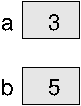
\includegraphics{figs/state.pdf}
\caption{Memory diagram of the variables \java{a} and \java{b}.}
\label{fig.state}
\end{center}
\end{figure}

\index{memory diagram}
\index{diagram!memory}

Diagrams like this one that show the state of the program are called {\bf memory diagrams}.
Each variable is represented with a box showing the name of the variable on the outside and the value inside.
As the program runs, the state of memory changes, so you should think of a state diagram as a snapshot of a particular point in time.


\section{Printing variables}
\label{sec:printvar}

You can display the current value of a variable using \java{print} or \java{println}.
The following statements declare a variable named \java{firstLine}, assign it the value \java{"Hello, again!"}, and display that value.

\begin{code}
String firstLine = "Hello, again!";
System.out.println(firstLine);
\end{code}

%Assuming this code fragment is inside a method that is inside a class, the output is:
%
%\begin{stdout}
%Hello, again!
%\end{stdout}

When we talk about displaying a variable, we generally mean the {\em value} of the variable.
To display the {\em name} of a variable, you have to put it in quotes.
%For example: \java{System.out.println("firstLine");}

\begin{code}
System.out.print("The value of firstLine is ");
System.out.println(firstLine);
\end{code}

For this example, the output is:

\begin{stdout}
The value of firstLine is Hello, again!
\end{stdout}

Conveniently, the syntax for displaying a variable is the same regardless of its type.
For example:

\begin{code}
int hour = 11;
int minute = 59;
System.out.print("The current time is ");
System.out.print(hour);
System.out.print(":");
System.out.print(minute);
System.out.println(".");
\end{code}

The output of this program is:

\begin{stdout}
The current time is 11:59.
\end{stdout}

To output multiple values on the same line, it's common to use several \java{print} statements followed by \java{println} at the end.
But don't forget the \java{println}!
On many computers, the output from \java{print} is stored without being displayed until \java{println} is run; then the entire line is displayed at once.
If you omit the \java{println}, the program might display the stored output at unexpected times or even terminate without displaying anything.


\section{Arithmetic operators}
\label{sec:arithops}

%Recall that Java programs are organized into {\em classes}, each of which has one or more {\em methods}, each of which has one or more {\em statements}.
%Most statements consist of one or more {\bf expressions}.

\index{operator}
\index{addition!integer}

{\bf Operators} are symbols that represent simple computations.
%Most operators in Java do what you expect them to do, since they are common mathematical symbols.
For example, the addition operator is \java{+}, subtraction is \java{-}, multiplication is \java{*}, and division is \java{/}.
%Variables are replaced with their values before the computation is performed.

The following program converts a time of day to minutes:

\begin{code}
int hour = 11;
int minute = 59;
System.out.print("Number of minutes since midnight: ");
System.out.println(hour * 60 + minute);
\end{code}

The output is:

\begin{stdout}
Number of minutes since midnight: 719
\end{stdout}

\index{expression}
\index{operand}

In this program, \java{hour * 60 + minute} is an {\bf expression}, which represents a single value to be computed (\java{719}).
When the program runs, each variable is replaced by its current value, and then the operators are applied.
The values that operators work with are called {\bf operands}.

Expressions are generally a combination of numbers, variables, and operators.
When compiled and executed, they become a single value.
For example, the expression \java{1 + 1} has the value \java{2}.
In the expression \java{hour - 1}, Java replaces the variable with its value, yielding \java{11 - 1}, which has the value \java{10}.

In the expression \java{hour * 60 + minute}, both variables get replaced, yielding \java{11 * 60 + 59}.
The multiplication happens first, yielding \java{660 + 59}.
Then the addition yields \java{719}.

Addition, subtraction, and multiplication all do what you expect, but you might be surprised by division.
For example, the following fragment tries to compute the fraction of an hour that has elapsed:%, but it has a logic error:

\begin{code}
System.out.print("Fraction of the hour that has passed: ");
System.out.println(minute / 60);
\end{code}

The output is:

\begin{stdout}
Fraction of the hour that has passed: 0
\end{stdout}

\index{division!integer}
\index{integer division}
\index{arithmetic!integer}

This result often confuses people.
The value of \java{minute} is 59, and 59 divided by 60 should be 0.98333, not 0.
The problem is that Java performs ``integer division'' when the operands are integers.
By design, integer division always rounds toward zero, even in cases like this one where the next integer is close.

As an alternative, we can calculate a percentage rather than a fraction:

\begin{code}
System.out.print("Percent of the hour that has passed: ");
System.out.println(minute * 100 / 60);
\end{code}

The new output is:

\begin{stdout}
Percent of the hour that has passed: 98
\end{stdout}

Again the result is rounded down, but at least now it's approximately correct.
%To get a more precise answer, we can use a different type of variable that can store fractional values.


\section{Floating-point numbers}

\index{floating-point}
\index{double}
\index{type!double}

A more general solution is to use {\bf floating-point} numbers, which can represent fractions as well as integers.
%As the name implies, the decimal point floats around (i.e., you can have as many decimal places as you want).
In Java, the default floating-point type is called \java{double}, which is short for double-precision.
You can create \java{double} variables and assign values to them using the same syntax we used for the other types:

\begin{code}
double pi;
pi = 3.14159;
\end{code}

Java performs ``floating-point division'' when one or more operands are \java{double} values.
So we can solve the problem we saw in the previous section:

\begin{code}
double minute = 59.0;
System.out.print("Fraction of the hour that has passed: ");
System.out.println(minute / 60.0);
\end{code}

The output is:

\begin{stdout}
Fraction of the hour that has passed: 0.9833333333333333
\end{stdout}

Although floating-point numbers are useful, they can be a source of confusion.
For example, Java distinguishes the integer value \java{1} from the floating-point value \java{1.0}, even though they seem to be the same number.
They belong to different data types, and strictly speaking, you are not allowed to make assignments between types.

The following is illegal because the variable on the left is an \java{int} and the value on the right is a \java{double}:

\begin{code}
int x = 1.1;  // compiler error
\end{code}

It is easy to forget this rule, because in many cases Java {\em automatically} converts from one type to another:

\begin{code}
double y = 1;  // legal, but bad style
\end{code}

The preceding example should be illegal, but Java allows it by converting the \java{int} value \java{1} to the \java{double} value \java{1.0} automatically.
This leniency is convenient, but it often causes problems for beginners.
For example:

\begin{code}
double y = 1 / 3;  // common mistake
\end{code}

\index{division!integer}
\index{integer division}
\index{arithmetic!integer}

You might expect the variable \java{y} to get the value \java{0.333333}, which is a legal floating-point value.
But instead it gets the value \java{0.0}.
The expression on the right divides two integers, so Java does integer division, which yields the \java{int} value \java{0}.
Converted to \java{double}, the value assigned to \java{y} is \java{0.0}.

One way to solve this problem (once you figure out the bug) is to make the right-hand side a floating-point expression.
The following sets \java{y} to \java{0.333333}, as expected:

\begin{code}
double y = 1.0 / 3.0;  // correct
\end{code}

As a matter of style, you should always assign floating-point values to floating-point variables.
The compiler won't make you do it, but you never know when a simple mistake will come back and haunt you.


\section{Rounding errors}

%The operations we have seen so far -- addition, subtraction, multiplication, and division -- also work on floating-point values, although you might be interested to know that the underlying mechanism is completely different.
%In fact, most processors have special circuitry just for performing floating-point operations.

Most floating-point numbers are only {\em approximately} correct.
Some numbers, like reasonably-sized integers, can be represented exactly.
But repeating fractions, like $1/3$, and irrational numbers, like $\pi$, cannot.
To represent these numbers, computers have to round off to the nearest floating-point number.

%Notwithstanding, there is a fundamental flaw with floating-point arithmetic.
%In mathematics, there is an infinite number of real numbers.
%But computer processors are finite; they cannot represent {\em every} possible floating-point number.
%Even with double-precision, you will frequently run into problems.

\index{rounding error}
\index{arithmetic!floating-point}

The difference between the number we want and the floating-point number we get is called {\bf rounding error}.
For example, the following two statements should be equivalent:

\begin{code}
System.out.println(0.1 * 10);
System.out.println(0.1 + 0.1 + 0.1 + 0.1 + 0.1
                 + 0.1 + 0.1 + 0.1 + 0.1 + 0.1);
\end{code}

But on many machines, the output is:

\begin{stdout}
1.0
0.9999999999999999
\end{stdout}

The problem is that \java{0.1}, which is a terminating fraction in decimal, is a repeating fraction in binary.
So its floating-point representation is only approximate.
When we add up the approximations, the rounding errors accumulate.

For many applications, like computer graphics, encryption, statistical analysis, and multimedia rendering, floating-point arithmetic has benefits that outweigh the costs.
But if you need {\em absolute} precision, use integers instead.
For example, consider a bank account with a balance of \$123.45:

\begin{code}
double balance = 123.45;  // potential rounding error
\end{code}

In this example, balances will become inaccurate over time as the variable is used in arithmetic operations like deposits and withdrawals.
The result would be angry customers and potential lawsuits.
You can avoid the problem by representing the balance as an integer:

\begin{code}
int balance = 12345;      // total number of cents
\end{code}

\index{type!long}

This solution works as long as the number of cents doesn't exceed the largest integer, which is about 2 billion.
%If necessary you can use \java{long} instead, which has a max value of $2^{63}-1$ (about 92 quadrillion dollars).
%Hopefully nobody will ever need that much money!


\section{Operators for strings}

\index{string!operator}
\index{operator!string}

In general, you cannot perform mathematical operations on strings, even if the strings look like numbers.
The following expressions are illegal:

\begin{code}
"Hello" - 1     "World" / 123     "Hello" * "World"
\end{code}

\index{concatenate}
\index{addition!string}

The \java{+} operator works with strings, but it might not do what you expect.
For strings, the \java{+} operator performs {\bf concatenation}, which means joining end-to-end.
So \java{"Hello, " + "World!"} yields the string \java{"Hello, World!"}.

Likewise if you have a variable called \java{name} that has type \java{String}, the expression \java{"Hello, " + name} appends the value of \java{name} to the hello string, which creates a personalized greeting.

Since addition is defined for both numbers and strings, Java performs automatic conversions you may not expect:

\begin{code}
System.out.println(1 + 2 + "Hello");
// the output is 3Hello

System.out.println("Hello" + 1 + 2);
// the output is Hello12
\end{code}

Java executes these operations from left to right.
In the first line, \java{1 + 2} is \java{3}, and \java{3 + "Hello"} is \java{"3Hello"}.
But in the second line, \java{"Hello" + 1} is \java{"Hello1"}, and \java{"Hello1" + 2} is \java{"Hello12"}.


%\section{Order of operations}

\index{order of operations}
\index{precedence}

When more than one operator appears in an expression, they are evaluated according to the {\bf order of operations}.
Generally speaking, Java evaluates operators from left to right (as we saw in the previous section).
But for numeric operators, Java follows mathematical conventions:

\begin{itemize}

\item Multiplication and division take ``precedence'' over addition and subtraction, which means they happen first.
So \java{1 + 2 * 3} yields 7, not 9, and \java{2 + 4 / 2} yields 4, not 3.

\item If the operators have the same precedence, they are evaluated from left to right.
So in the expression \java{minute * 100 / 60}, the multiplication happens first; if the value of \java{minute} is 59, we get \java{5900 / 60}, which yields \java{98}.
If these same operations had gone from right to left, the result would have been \java{59 * 1}, which is incorrect.

\item Any time you want to override the order of operations (or you are not sure what it is) you can use parentheses.
Expressions in parentheses are evaluated first, so \java{(1 + 2) * 3} is 9.
You can also use parentheses to make an expression easier to read, as in \java{(minute * 100) / 60}, even though it doesn't change the result.

\end{itemize}

Don't work too hard to remember the order of operations, especially for other operators.
If it's not obvious by looking at the expression, use parentheses to make it clear.


\section{Composition}

\index{composition}

So far we have looked at the elements of a programming language -- variables, expressions, and statements -- in isolation, without talking about how to put them together.

One of the most useful features of programming languages is their ability to take small building blocks and {\bf compose} them.
For example, we know how to multiply numbers and we know how to display values.
We can combine these operations into a single statement:

\begin{code}
System.out.println(17 * 3);
\end{code}

Any arithmetic expression can be used inside a print statement.
We've already seen one example:

\begin{code}
System.out.println(hour * 60 + minute);
\end{code}

You can also put arbitrary expressions on the right side of an assignment:

\begin{code}
int percentage;
percentage = (minute * 100) / 60;
\end{code}

The left side of an assignment must be a variable name, not an expression.
That's because the left side indicates where the result will be stored, and expressions do not represent storage locations.

\begin{code}
hour = minute + 1;  // correct
minute + 1 = hour;  // compiler error
\end{code}

\index{readability}

The ability to compose operations may not seem impressive now, but we will see examples later on that allow us to write complex computations neatly and concisely.
But don't get too carried away.
Large, complex expressions can be hard to read and debug.

%Before you get too carried away with composition, keep in mind that other people will be reading your source code.
%In practice, software developers spend the vast majority of their time {\em understanding} and {\em modifying} existing code.
%Thus it's far more important to write code that is readable than to write code that is (or appears to be) optimal.
%There is much beauty in simplicity.
%In general, each line of code should be a single step of the algorithm.


\section{Types of errors}

\index{error!message}

Three kinds of errors can occur in a program: compile-time errors, run-time errors, and logic errors.
It is useful to distinguish among them in order to track them down more quickly.

\index{compile-time error}
\index{error!compile-time}

{\bf Compile-time} errors occur when you violate the syntax rules of the Java language.
For example, parentheses and braces have to come in matching pairs.
So \java{(1 + 2)} is legal, but \java{8)} is not.
In the latter case, the program cannot be compiled, and the compiler displays an error.

\index{error!message}

Error messages from the compiler usually indicate where in the program the error occurred, and sometimes they can tell you exactly what the error is.
As an example, let's get back to the hello world program from Section~\ref{hello}.

\begin{trinket}[235]{Hello.java}
public class Hello {

    public static void main(String[] args) {
        // generate some simple output
        System.out.println("Hello, World!");
    }
}
\end{trinket}

\index{semicolon}

If you forget the semicolon at the end of the print statement, you might get an error message like this:

\begin{stdout}
File: Hello.java  [line: 5]
Error: ';' expected
\end{stdout}

That's pretty good: the location of the error is correct, and the error message tells you what's wrong.

But error messages are not always easy to understand.
Sometimes the compiler reports the place in the program where the error was {\em detected}, not where it actually occurred.
And sometimes the description of the problem is more confusing than helpful.

For example, if you forget the closing brace at the end of \java{main} (line 6), you might get a message like this:

\begin{stdout}
File: Hello.java  [line: 7]
Error: reached end of file while parsing
\end{stdout}

\index{parse}

There are two problems here.
First, the error message is written from the compiler's point of view, not yours.
{\bf Parsing} is the process of reading a program before translating; if the compiler gets to the end of the file while still parsing, that means something was omitted.
But the compiler doesn't know what.
It also doesn't know where.
The compiler discovers the error at the end of the program (line 7), but the missing brace should be on the previous line.

Error messages contain useful information, so you should make an effort to read and understand them.
But don't take them too literally.
During the first few weeks of your programming career, you will probably spend a lot of time tracking down compile-time errors.
As you gain experience, you will make fewer mistakes and find them more quickly.

%\subsection{Run-time errors}

\index{run-time error}
\index{error!run-time}
\index{exception}

The second type of error is a {\bf run-time error}, so-called because it does not appear until after the program has started running.
In Java, these errors occur while the interpreter is executing byte code and something goes wrong.
These errors are also called ``exceptions'' because they usually indicate that something unexpected has happened.

Run-time errors are rare in the simple programs you will see in the first few chapters, so it might be a while before you encounter one.
When a run-time error occurs, the interpreter displays an error message that explains what happened and where.
For example, if you accidentally divide by zero you will get a message like:

\begin{small}
\begin{stdout}
Exception in thread "main" java.lang.ArithmeticException: / by zero
    at Hello.main(Hello.java:5)
\end{stdout}
\end{small}

\index{ArithmeticException}
\index{exception!Arithmetic}

Error messages are very useful for debugging.
The first line includes the name of the exception, \java{java.lang.ArithmeticException}, and a message that indicates more specifically what happened, \java{/ by zero}.
The next line shows the method where the error occurred; \java{Hello.main} indicates the method \java{main} in the class \java{Hello}.
It also reports the file where the method is defined, {\tt Hello.java}, and the line number where the error occurred, \java{5}.

Sometimes error messages contain additional information that doesn't make sense.
It can be a challenge to figure out where to find the useful parts without being overwhelmed by extraneous information.
Keep in mind that the line where the program crashed may not be the line that needs to be corrected.

%\subsection{Logic errors}

\index{logic error}
\index{error!logic}

The third type of error is a {\bf logic error}.
%{\bf Semantics} pertains to the meaning of a program; that is, what it does when it runs.
If your program has a logic error, it will compile and run without generating error messages, but it will not do the right thing.
Instead, it will do exactly what you told it to do.
For example, here is a version of the hello world program with a logic error:

\begin{trinket}[235]{Hello.java}
public class Hello {

    public static void main(String[] args) {
        System.out.println("Hello, ");
        System.out.println("World!");
    }
}
\end{trinket}

This program compiles and runs just fine, but the output is:

\begin{stdout}
Hello,
World!
\end{stdout}

Assuming that we wanted the output on one line, this is not correct.
The problem is that the first line uses \java{println}, when we probably meant to use \java{print} (see the ``goodbye world'' example of Section~\ref{goodbye}).

Identifying logic errors can be hard because you have to work backwards, looking at the output of the program, trying to figure out why it is doing the wrong thing, and how to make it do the right thing.
Usually the compiler and the interpreter can't help you, since they don't know what the right thing is.

Now that you know about the three kinds of errors, you might want to preview Appendix~\ref{debugappendix} where we've collected some of our favorite debugging advice.
It refers to language features we haven't talked about yet, so you will want to re-read it from time to time.


\section{Vocabulary}

\begin{description}

\term{variable}
A named storage location for values.
All variables have a type, which is declared when the variable is created.

\term{value}
A number, string, or other data that can be stored in a variable.
Every value belongs to a type (for example, \java{int} or \java{String}).

\term{declaration}
A statement that creates a new variable and specifies its type.

\term{type}
Mathematically speaking, a set of values.
The type of a variable determines which values it can have.

\term{syntax}
The structure of a program; the arrangement of the words and symbols it contains.

\term{keyword}
A reserved word used by the compiler to analyze programs.
You cannot use keywords (like \java{public}, \java{class}, and \java{void}) as variable names.

\term{assignment}
A statement that gives a value to a variable.

\term{initialize}
To assign a variable for the first time.

%\term{update}
%An assignment that changes the value of a variable.

\term{state}
The variables in a program and their current values.

\term{memory diagram}
A graphical representation of the state of a program at a point in time.

\term{operator}
A symbol that represents a computation like addition, multiplication, or string concatenation.

\term{operand}
One of the values on which an operator operates.
Most operators in Java require two operands.

\term{expression}
A combination of variables, operators, and values that represents a single value.
Expressions also have types, as determined by their operators and operands.

\term{floating-point}
A data type that represents numbers with an integer part and a fractional part.
In Java, the default floating-point type is \java{double}.

\term{rounding error}
The difference between the number we want to represent and the nearest floating-point number.

\term{concatenate}
To join two values, often strings, end-to-end.

\term{order of operations}
The rules that determine in what order operations are evaluated.

\term{composition}
The ability to combine simple expressions and statements into compound expressions and statements.

\term{compile-time error}
An error in the source code that makes it impossible to compile.
Also called a ``syntax error''.

\term{parse}
To analyze the structure of a program; what the compiler does first.

\term{run-time error}
An error in a program that makes it impossible to run to completion.
Also called an ``exception''.

\term{logic error}
An error in a program that makes it do something other than what the programmer intended.

%\term{semantics}
%The meaning of a program; the low-level instructions it should perform.

\end{description}


\section{Exercises}

The code for this chapter is in the {\tt ch02} directory of {\tt ThinkJava2Code}.
See page~\pageref{code} for instructions on how to download the repository.
Before you start the exercises, we recommend that you compile and run the examples.

If you have not already read Appendix~\ref{interactions}, now might be a good time.
It describes the DrJava Interactions Pane, which is a useful way to develop and test short fragments of code without writing a complete class definition.


\begin{exercise}

If you are using this book in a class, you might enjoy this exercise.
Find a partner and play ``Stump the Chump'':

Start with a program that compiles and runs correctly.
One player looks away while the other player adds an error to the program.
Then the first player tries to find and fix the error.
You get two points if you find the error without compiling the program, one point if you find it using the compiler, and your opponent gets a point if you don't find it.

\end{exercise}


\begin{exercise}
\label{ex:date}

The point of this exercise is (1) to use string concatenation to display values with different types (\java{int} and \java{String}), and (2) to practice developing programs gradually by adding a few statements at a time.

\begin{enumerate}

\item Create a new program named {\tt Date.java}.
Copy or type in something like the hello world program and make sure you can compile and run it.

\item Following the example in Section~\ref{sec:printvar}, write a program that creates variables named \java{day}, \java{date}, \java{month}, and \java{year}.
The variable \java{day} will contain the day of the week (like Friday), and \java{date} will contain the day of the month (like the 13th).
What type is each variable?
Assign values to those variables that represent today's date.

\item Display (print out) the value of each variable on a line by itself.
This is an intermediate step that is useful for checking that everything is working so far.
Compile and run your program before moving on.

\item Modify the program so that it displays the date in standard American format, for example: {\tt Thursday, July 16, 2015}.

\item Modify the program so it also displays the date in European format.
The final output should be:

\begin{stdout}
American format:
Thursday, July 16, 2015
European format:
Thursday 16 July 2015
\end{stdout}

%{\it Hint:} You should be able to copy, paste, and modify the code from Step 4 when completing Step 5.
\end{enumerate}

\end{exercise}


\begin{exercise}

The point of this exercise is to (1) use some of the arithmetic operators, and (2) start thinking about compound entities (like time of day) that are represented with multiple values.

\begin{enumerate}

\item Create a new program called {\tt Time.java}.
From now on, we won't remind you to start with a small, working program, but you should.

\item Following the example program in Section~\ref{sec:printvar}, create variables named \java{hour}, \java{minute}, and \java{second}.
Assign values that are roughly the current time.
Use a 24-hour clock so that at 2pm the value of \java{hour} is 14.

\item Make the program calculate and display the number of seconds since midnight.

\item Calculate and display the number of seconds remaining in the day.

\item Calculate and display the percentage of the day that has passed.
You might run into problems when computing percentages with integers, so consider using floating-point.

\item Change the values of \java{hour}, \java{minute}, and \java{second} to reflect the current time.
Then write code to compute the elapsed time since you started working on this exercise.

\end{enumerate}

{\it Hint:} You might want to use additional variables to hold values during the computation.
Variables that are used in a computation but never displayed are sometimes called ``intermediate'' or ``temporary'' variables.

\end{exercise}
